%  LaTeX support: latex@mdpi.com 
%  In case you need support, please attach all files that are necessary for compiling as well as the log file, and specify the details of your LaTeX setup (which operating system and LaTeX version / tools you are using).

%=================================================================
\documentclass[materials,article,submit,moreauthors,pdftex]{Definitions/mdpi} 
% If you would like to post an early version of this manuscript as a preprint, you may use preprint as the journal and change 'submit' to 'accept'. The document class line would be, e.g., \documentclass[preprints,article,accept,moreauthors,pdftex]{mdpi}. This is especially recommended for submission to arXiv, where line numbers should be removed before posting. For preprints.org, the editorial staff will make this change immediately prior to posting.

%--------------------
% Class Options:
%--------------------
%----------
% journal
%----------
% Choose between the following MDPI journals:
% acoustics, actuators, addictions, admsci, aerospace, agriculture, agriengineering, agronomy, algorithms, animals, antibiotics, antibodies, antioxidants, applsci, arts, asc, asi, atmosphere, atoms, axioms, batteries, bdcc, behavsci , beverages, bioengineering, biology, biomedicines, biomimetics, biomolecules, biosensors, brainsci , buildings, cancers, carbon , catalysts, cells, ceramics, challenges, chemengineering, chemistry, chemosensors, children, cleantechnol, climate, clockssleep, cmd, coatings, colloids, computation, computers, condensedmatter, cosmetics, cryptography, crystals, dairy, data, dentistry, designs , diagnostics, diseases, diversity, drones, econometrics, economies, education, ejihpe, electrochem, electronics, energies, entropy, environments, epigenomes, est, fermentation, fibers, fire, fishes, fluids, foods, forecasting, forests, fractalfract, futureinternet, futurephys, galaxies, games, gastrointestdisord, gels, genealogy, genes, geohazards, geosciences, geriatrics, hazardousmatters, healthcare, heritage, highthroughput, horticulturae, humanities, hydrology, ijerph, ijfs, ijgi, ijms, ijns, ijtpp, informatics, information, infrastructures, inorganics, insects, instruments, inventions, iot, j, jcdd, jcm, jcp, jcs, jdb, jfb, jfmk, jimaging, jintelligence, jlpea, jmmp, jmse, jnt, jof, joitmc, jpm, jrfm, jsan, land, languages, laws, life, literature, logistics, lubricants, machines, magnetochemistry, make, marinedrugs, materials, mathematics, mca, medicina, medicines, medsci, membranes, metabolites, metals, microarrays, micromachines, microorganisms, minerals, modelling, molbank, molecules, mps, mti, nanomaterials, ncrna, neuroglia, nitrogen, notspecified, nutrients, ohbm, optics, particles, pathogens, pharmaceuticals, pharmaceutics, pharmacy, philosophies, photonics, physics, plants, plasma, polymers, polysaccharides, preprints , proceedings, processes, proteomes, psych, publications, quantumrep, quaternary, qubs, reactions, recycling, religions, remotesensing, reports, resources, risks, robotics, safety, sci, scipharm, sensors, separations, sexes, signals, sinusitis, smartcities, sna, societies, socsci, soilsystems, sports, standards, stats, surfaces, surgeries, sustainability, symmetry, systems, technologies, test, toxics, toxins, tropicalmed, universe, urbansci, vaccines, vehicles, vetsci, vibration, viruses, vision, water, wem, wevj

%---------
% article
%---------
% The default type of manuscript is "article", but can be replaced by: 
% abstract, addendum, article, benchmark, book, bookreview, briefreport, casereport, changes, comment, commentary, communication, conceptpaper, conferenceproceedings, correction, conferencereport, expressionofconcern, extendedabstract, meetingreport, creative, datadescriptor, discussion, editorial, essay, erratum, hypothesis, interestingimages, letter, meetingreport, newbookreceived, obituary, opinion, projectreport, reply, retraction, review, perspective, protocol, shortnote, supfile, technicalnote, viewpoint
% supfile = supplementary materials

%----------
% submit
%----------
% The class option "submit" will be changed to "accept" by the Editorial Office when the paper is accepted. This will only make changes to the frontpage (e.g., the logo of the journal will get visible), the headings, and the copyright information. Also, line numbering will be removed. Journal info and pagination for accepted papers will also be assigned by the Editorial Office.

%------------------
% moreauthors
%------------------
% If there is only one author the class option oneauthor should be used. Otherwise use the class option moreauthors.

%---------
% pdftex
%---------
% The option pdftex is for use with pdfLaTeX. If eps figures are used, remove the option pdftex and use LaTeX and dvi2pdf.

%=================================================================
\firstpage{1} 
\makeatletter 
\setcounter{page}{\@firstpage} 
\makeatother
\pubvolume{xx}
\issuenum{1}
\articlenumber{5}
\pubyear{2020}
\copyrightyear{2020}
%\externaleditor{Academic Editor: name}
\history{Received: date; Accepted: date; Published: date}
%\updates{yes} % If there is an update available, un-comment this line

%% MDPI internal command: uncomment if new journal that already uses continuous page numbers 
%\continuouspages{yes}

%------------------------------------------------------------------
% The following line should be uncommented if the LaTeX file is uploaded to arXiv.org
%\pdfoutput=1

%=================================================================
% Add packages and commands here. The following packages are loaded in our class file: fontenc, calc, indentfirst, fancyhdr, graphicx, lastpage, ifthen, lineno, float, amsmath, setspace, enumitem, mathpazo, booktabs, titlesec, etoolbox, amsthm, hyphenat, natbib, hyperref, footmisc, geometry, caption, url, mdframed, tabto, soul, multirow, microtype, tikz
\usepackage[ruled,vlined]{algorithm2e}
%=================================================================
%% Please use the following mathematics environments: Theorem, Lemma, Corollary, Proposition, Characterization, Property, Problem, Example, ExamplesandDefinitions, Hypothesis, Remark, Definition, Notation, Assumption
%% For proofs, please use the proof environment (the amsthm package is loaded by the MDPI class).

%=================================================================
% Full title of the paper (Capitalized)
\Title{Model-Assisted Guided-Wave Based Approach for Disbonds Detection in Honeycomb Sandwich Structures}

% Author Orchid ID: enter ID or remove command
\newcommand{\orcidauthorA}{0000-0002-5030-3312} % Add \orcidA{} behind the author's name
\newcommand{\orcidauthorB}{0000-0002-5130-6443} % Add \orcidB{} behind the author's name

% Authors, for the paper (add full first names)
\Author{Piotr Fiborek*\orcidA{} and Pawe\l{} Kudela\orcidB{}}

% Authors, for metadata in PDF
\AuthorNames{Piotr Fiborek and Pawe\l{} Kudela}

% Affiliations / Addresses (Add [1] after \address if there is only one affiliation.)
\address[1]{%
Institute of Fluid Flow Machinery, Polish Academy of Sciences,  imp@imp.gda.pl}

% Contact information of the corresponding author
\corres{Correspondence: pfiborek@imp.gda.pl}

% Current address and/or shared authorship

% The commands \thirdnote{} till \eighthnote{} are available for further notes

%\simplesumm{} % Simple summary

%\conference{} % An extended version of a conference paper

% Abstract (Do not insert blank lines, i.e. \\) 
\abstract{One of the axioms of the structural health monitoring states that the severity of damage assessment can only be done in a learning mode under the supervision of an expert.
Therefore, a numerical analysis will be conducted to gain knowledge about the influence of the damage size on the propagation of elastic waves in the honeycomb sandwich composite panel.
For this purpose, a panel has been modelled taking into account the real geometry of the honeycomb core using the time-domain spectral element method and two-dimensional elements.
The presented model was compared with the homogenised model of the honeycomb core.
The damage under investigation was the disbond between the skin and the core of the panel.
The use of two-dimensional elements required connecting the nodes of adjacent elements, which was realised through an interface based on Lagrange multipliers.
The result of the parametric study is a function of damage influence on the amplitude of propagating waves.}

% Keywords
\keyword{honeycomb sandwich structures; spectral element method; structural health monitoring; guided waves}

% The fields PACS, MSC, and JEL may be left empty or commented out if not applicable
%\PACS{J0101}
%\MSC{}
%\JEL{}

%%%%%%%%%%%%%%%%%%%%%%%%%%%%%%%%%%%%%%%%%%
% Only for the journal Diversity
%\LSID{\url{http://}}

%%%%%%%%%%%%%%%%%%%%%%%%%%%%%%%%%%%%%%%%%%
% Only for the journal Applied Sciences:
%\featuredapplication{Authors are encouraged to provide a concise description of the specific application or a potential application of the work. This section is not mandatory.}
%%%%%%%%%%%%%%%%%%%%%%%%%%%%%%%%%%%%%%%%%%

%%%%%%%%%%%%%%%%%%%%%%%%%%%%%%%%%%%%%%%%%%
% Only for the journal Data:
%\dataset{DOI number or link to the deposited data set in cases where the data set is published or set to be published separately. If the data set is submitted and will be published as a supplement to this paper in the journal Data, this field will be filled by the editors of the journal. In this case, please make sure to submit the data set as a supplement when entering your manuscript into our manuscript editorial system.}

%\datasetlicense{license under which the data set is made available (CC0, CC-BY, CC-BY-SA, CC-BY-NC, etc.)}

%%%%%%%%%%%%%%%%%%%%%%%%%%%%%%%%%%%%%%%%%%
% Only for the journal Toxins
%\keycontribution{The breakthroughs or highlights of the manuscript. Authors can write one or two sentences to describe the most important part of the paper.}

%\setcounter{secnumdepth}{4}
%%%%%%%%%%%%%%%%%%%%%%%%%%%%%%%%%%%%%%%%%%
\begin{document}
%%%%%%%%%%%%%%%%%%%%%%%%%%%%%%%%%%%%%%%%%%
\section{Introduction}
\label{sec:intro}
Honeycomb Sandwich Composite~(HSC) is a type of multi-layered structure, which is composed of the mid-core with the geometry of honeycomb sandwiched between thin skins.
They are widely used in the aerospace, marine and automotive industries due to the high strength-to-weight ratio, high energy absorption capability and effective acoustic insulation.
However, these complex structures are exposed to various types of damage that are not found in metal alloy materials, e.g. hidden disbonds between the skin and the core, delamination of the skin plates, or the core impact damage.
They can occur either during a manufacturing process, storage or in-service life.
Therefore, advanced methods are required for on-line damage detections.

The structural health monitoring (SHM) method with very high potential is the method based on the Guided Wave (GW) propagation \cite{mustapha2011assessment, sikdar2016guided, sikdar2016ultrasonic,radzienski2016assessment, yu2019core}.
GW are mechanical waves that propagate in a bounded, elastic medium, e.g. bars, beams, rods, plates and shells.
The wavelength of GW is longer than the thickness of the bounding elastic medium.
An excitation and sensing of the GW can be realised by the lightweight and inexpensive piezoelectric transducers (PZT) \cite{giurgiutiumicromechatronics}.
The compact PZT can be surface-bonded to the inspected structure or even embedded between the composite plies so that the measurements can be conducted in situ.
Among numerous techniques developed for damage detection and localisation, the most popular are pitch--catch \cite{ihn2008pitch, sikdar2017structural}, pulse--echo \cite{guo1993interaction, kudela2008damage}, phase array \cite{lu2006crack, ostachowicz2008elastic}, and time-reversal mirror \cite{fink1992time, eremin2016analytically}.
	
The most common numerical modelling of the phenomenon of GW in HSC found in the literature is a calculation of the effective material properties of the honeycomb structure by the homogenisation process~\cite{shi1995derivation, qi2008ultrasonic, mustapha2014leaky, baid2015dispersion, sikdar2016guided}.
However, this method is not able to adequately present the phenomenon of propagation of elastic waves in such material.
A more accurate model will be achieved if the real geometry of the hexagonal cell is retained.
	
Ruzzenne et al. presented a parametric study to evaluate the dynamic behaviour of the honeycomb and cellular structures through the finite element model and the application of the theory of periodic structures \cite{ruzzene2003wave}.
Recently, the simulations of the wave propagation in the HSC have been conducted with the commercially available finite element code~\cite{song2009guided, hosseini2013numerical, tian2015wavenumber, zhao2018wave}.
However, the finite element method (FEM) of GW are inefficient as they require a significant amount of memory and are time-consuming.

The computational efficiency of the FEM in case of GW modelling in the HSC can be improved by using the time-domain spectral element method (SEM).
The SEM was originally used for the numerical solution of the fluid--flow in a channel by Patera \cite{patera1984spectral} but has also been successfully developed for elastic wave propagation~\cite{ostachowicz2011guided}.
Kudela proposed a model of the GW in HSC by the parallel implementation of the SEM \cite{kudela2016parallel}.
However, this model had a large number (1.5 million) of degrees-of-freedom (DOF), because cells of the core and skin plate were modelled by the three-dimensional (3D) spectral elements.
Although, the simulation was limited to only one skin plate and a small dimension of the HSC (\(179 \times 159 \) mm).

Above mentioned drawbacks were motivation to propose a new model of the HSC. In the present paper, the skin plates, adhesive layers and each wall of the hexagonal core were modelled by two-dimensional (2D) spectral elements.
However, 2D elements have nodes only in a mid-plane, therefore, there is no direct connection between the two adjacent structures.
This connection was implemented by interface elements based on Lagrange multipliers \cite{ashwin2014formulation, fiborek20192d}.
Additionally, the signal was generated and recorded with piezoelectric transducers (PZT), while Kudela excited the waves with an external force applied at the point of the panel \cite{kudela2016parallel}.
A non-matching interface between the transducers and the skin was used to avoid too complex mesh, likewise to the interfaces developed for the FEM \cite{flemisch2000elasto, flemisch2012non}. To the best of authors’
knowledge, it has not been implemented for the SEM.

The parametric study conducted in the paper leads to the determination of a model-assisted damage identification function (MADIF), which determines the influence of the size of the composite defect on wave propagation.
In this case, the defect is assumed to be a disbond between the skin and the core.

\section{The time-domain spectral element method formulation}
\label{sec:time_SEM}
\subsection{The spectral element method}
\label{sec:sem}
The general concept of the SEM is based on the idea of the FEM.
The similarity of both methods lies in the fact that the modelled domain is divided into non-overlapping finite elements, and external forces and arbitrary boundary conditions are imposed in the particular nodes.
The main difference between those methods is a choice of the shape function \( N=N(\xi )\), which is interpolated by Lagrange polynomial that passes through the element nodes. The nodes are localized on the endpoint of an interval, \(\xi\in[-1,1]\) and the roots of the first derivative of Legendre polynomial of degree \(p-1\):

\begin{eqnarray}
(1-\xi^2)P'_{p-1}(\xi)=0
\label{eq:nodes}
\end{eqnarray}

The approximation of an integral over the elements is achieved according to Gauss-Lobatto-Legendre (GLL) rule at points coinciding with the element nodes, 
and the weights \(w=w(\xi)\) calculated as:
\begin{eqnarray}
{w(\xi)} = \frac{2}{p(p-1)(P_{p-1}(\xi))^2}
\label{eq:weights}
\end{eqnarray}
This approach guarantees a diagonal mass matrix.
The shape functions and the weights for 2D or 3D elements are obtained by the Kronecker product of vectors of individual axes, denoted by \(\otimes\) as follows:
\begin{eqnarray}
N(\xi,\eta) = N(\xi)\otimes N(\eta), & N(\xi,\eta,\zeta) = N(\xi)\otimes N(\eta)\otimes N(\zeta) \nonumber\\
w(\xi,\eta) = w(\xi)\otimes w(\eta), & w(\xi,\eta,\zeta) = w(\xi)\otimes w(\eta)\otimes w(\zeta) 
\label{eq:3Dshape_weights}
\end{eqnarray}
\subsection{2D spectral modelling}
\label{sec:2D_SEM}

According to the first-order shear deformation theory~\cite{reissner1945effect, mindlin1951influence} the vector of displacements is expressed as:
\begin{eqnarray}
\left \{ \begin{array}{c}
\textbf{u}^e(\xi,\eta,\zeta) \\
\textbf{v}^e(\xi,\eta,\zeta) \\
\textbf{w}^e(\xi,\eta,\zeta)
\end{array} \right\} = 
\left \{ \begin{array}{c}
\textbf{u}_0^e(\xi,\eta) + z\boldsymbol{\varphi}_x^e(\xi,\eta)\\
\textbf{v}_0^e(\xi,\eta) + z\boldsymbol{\varphi}_y^e(\xi,\eta)\\
\textbf{w}_0^e(\xi,\eta) \\
\end{array} \right\}
\end{eqnarray}
where \(\textbf{u}_0^e\), \(\textbf{v}_0^e\) and \(\textbf{w}_0^e\) are nodal displacements, \(\boldsymbol{\varphi}_x^e\), \(\boldsymbol{\varphi}_y^e\) are the rotations of the normal to the mid-plane with respect to axes \textit{x} and \textit{y}, respectively.
\begin{eqnarray}
\left \{\begin{array}{c}
\textbf{u}_0^e(\xi,\eta) \\
\textbf{v}_0^e(\xi,\eta) \\
\textbf{w}_0^e(\xi,\eta) \\
\boldsymbol{\varphi}_x^e(\xi,\eta) \\
\boldsymbol{\varphi}_y^e(\xi,\eta)
\end{array} \right\}
& = & \textbf{N}^e(\xi,\eta)\widehat{\textbf{d}}^e\nonumber\\
& = & \sum_{n=1}^q\sum_{m=1}^p\textbf{N}_m^e(\xi)\textbf{N}_n^e(\eta)
\left [ \begin{array}{c}
\widehat{\textbf{u}}_0^e \\
\widehat{\textbf{v}}_0^e \\
\widehat{\textbf{w}}_0^e \\
\widehat{\boldsymbol{\varphi}}_x^e \\
\widehat{\boldsymbol{\varphi}}_y^e
\end{array} \right]
\end{eqnarray}
The nodal bending strain-displacement relations are given in the form:
\begin{eqnarray}
\boldsymbol{\epsilon}_b^e =
\textbf{B}_b^e\widehat{\textbf{d}}^e = 
\left [
\begin{array}{ccccc}
\frac{\partial N^e}{\partial x} & 0 & 0 & 0 & 0\\
0 & \frac{\partial N^e}{\partial y} & 0 & 0 & 0\\
\frac{\partial N^e}{\partial y} & \frac{\partial N^e}{\partial x} & 0 & 0 & 0\\
0 & 0 & 0 & -\frac{\partial N^e}{\partial x} & 0\\
0 & 0 & 0 & 0 & -\frac{\partial N^e}{\partial y}\\
0 & 0 & 0 & -\frac{\partial N^e}{\partial y} & -\frac{\partial N^e}{\partial x}
\end{array} \right]
\left \{ \begin{array}{c}
\textbf{u}_0^e \\
\textbf{v}_0^e \\
\textbf{w}_0^e \\
\boldsymbol{\varphi}_x^e \\
\boldsymbol{\varphi}_y^e
\end{array} \right\}
\end{eqnarray}
The nodal shear strain-displacement relations are given in the form:
\begin{eqnarray}
\boldsymbol{\epsilon}_s^e =
\textbf{B}_s^e\widehat{\textbf{d}}^e = 
\left [
\begin{array}{ccccc}
0 & 0 & \frac{\partial N^e}{\partial y} & -1 & 0\\
0 & 0 & \frac{\partial N^e}{\partial y} & 0 & -1
\end{array} \right]
\left \{ \begin{array}{c}
\textbf{u}_0^e \\
\textbf{v}_0^e \\
\textbf{w}_0^e \\
\boldsymbol{\varphi}_x^e \\
\boldsymbol{\varphi}_y^e
\end{array} \right\}
\end{eqnarray}
\subsection{3D model of the PZT transducer}
\label{sec:3D_SEM}
The displacements vector of the PZT transducer is composed of three translational displacements, and it is defined as:
\begin{eqnarray}
\left \{ \begin{array}{c}
\textbf{u}^e(\xi,\eta,\zeta) \\
\textbf{v}^e(\xi,\eta,\zeta) \\
\textbf{w}^e(\xi,\eta,\zeta)
\end{array} \right\}
& = & \textbf{N}^e(\xi,\eta, \zeta)\widehat{\textbf{d}}^e\nonumber\\
& = & \sum_{l=1}^r\sum_{n=1}^q\sum_{m=1}^p\textbf{N}_m^e(\xi)\textbf{N}_n^e(\eta)\textbf{N}_l^e(\zeta)
\left \{ \begin{array}{c}
\widehat{\textbf{u}}^e(\xi_m,\eta_n,\zeta_l) \\
\widehat{\textbf{v}}^e(\xi_m,\eta_n,\zeta_l) \\
\widehat{\textbf{w}}^e(\xi_m,\eta_n,\zeta_l)
\end{array} \right\}
\label{eq:3D_displ}
\end{eqnarray}
where \(\widehat{\textbf{u}}^e\), \(\widehat{\textbf{v}}^e\) and 
\(\widehat{\textbf{w}}^e\) are displacements of the element nodes in \(\xi,\eta\) and \(\zeta\) direction.

The nodal strain-displacement relations are given as \cite{kudela20093d}:
\begin{eqnarray}
\boldsymbol{\epsilon}^e=\textbf{B}_{d}^e\widehat{\textbf{d}}^e=
\left [
\begin{array}{ccc}
\frac{\partial N^e}{\partial x} & 0 & 0\\
0 & \frac{\partial N^e}{\partial y} & 0\\
0 & 0 & \frac{\partial N^e}{\partial z}\\
0 & \frac{\partial N^e}{\partial z} & \frac{\partial N^e}{\partial y}\\
\frac{\partial N^e}{\partial z} & 0 & \frac{\partial N^e}{\partial x}\\
\frac{\partial N^e}{\partial y} & \frac{\partial N^e}{\partial x} & 0
\end{array} \right]
\left \{ \begin{array}{c}
\textbf{u}^e \\
\textbf{v}^e \\
\textbf{w}^e
\end{array} \right\}
\end{eqnarray}

The electromechanical coupling is governed by the linear constitutive equation of piezoelectric material according to~\cite{giurgiutiumicromechatronics, rekatsinas2017cubic}, and it is defined as:
\begin{eqnarray}
\left [ 
\begin {array}{c}
\boldsymbol{\sigma}\\
\textbf{D}
\end{array}\right ]=
\left [ 
\begin{array}{cc}
\textbf{c}^E & -\textbf{e}^T \\
\textbf{e} & \epsilon^S 
\end{array} \right ]
\left[ 
\begin{array}{c}
\textbf{S}\\
\textbf{E} 
\end{array} \right ]
\end{eqnarray}
where \(\textbf{c}^E\) is the stiffness coefficients measured at zero electric field, \textbf{e} is the piezoelectric coupling tensor and \(\boldsymbol{\epsilon}^S\) electric permittivity, \textbf{E} and \textbf{D} are the electric field and electric displacement measured at zero strain.
The superscript T denotes transpose matrix.
The eElectric field is defined as:
\begin{eqnarray}
\textbf{E}^e=-\textbf{B}_\phi^e \widehat{\phi}^e = \left[ \begin{array}{c}
\frac{\partial N^e}{\partial \xi}\\
\frac{\partial N^e}{\partial \eta}\\
\frac{\partial N^e}{\partial \zeta}
\end{array} \right] \widehat{\phi}^e
\end{eqnarray}

\subsection{Displacements coupling at the substructures interface}
\label{sec:interface}
The present model of the sandwich panel consists of 2D and 3D elements. 
Moreover, there are non-matching grids between two adjacent substructures. 
These involve connecting them by imposing the compatibility of the displacements at the interface, see Fig.~\ref{fig:interface}.
This type of connection is implemented through the interface elements based on Lagrange multipliers, which are interpreted as forces responsible for determining the appropriate displacements of nodes.
The coupling can be expressed as:
\begin{eqnarray}
\left\{\begin{array}{c}
\textbf{u}\\
\textbf{v}\\
\textbf{w}
\end{array}\right\}_{s_{i1}}^{\Gamma^i}-
\left\{\begin{array}{c}
\textbf{u}\\
\textbf{v}\\
\textbf{w}
\end{array}\right\}_{s_{i2}}^{\Gamma^i}=
\left\{\begin{array}{c}
\textbf{0}\\
\textbf{0}\\
\textbf{0}
\end{array}\right\}
\label{eq:coupling}
\end{eqnarray}
\begin{figure}
	\begin{center}
		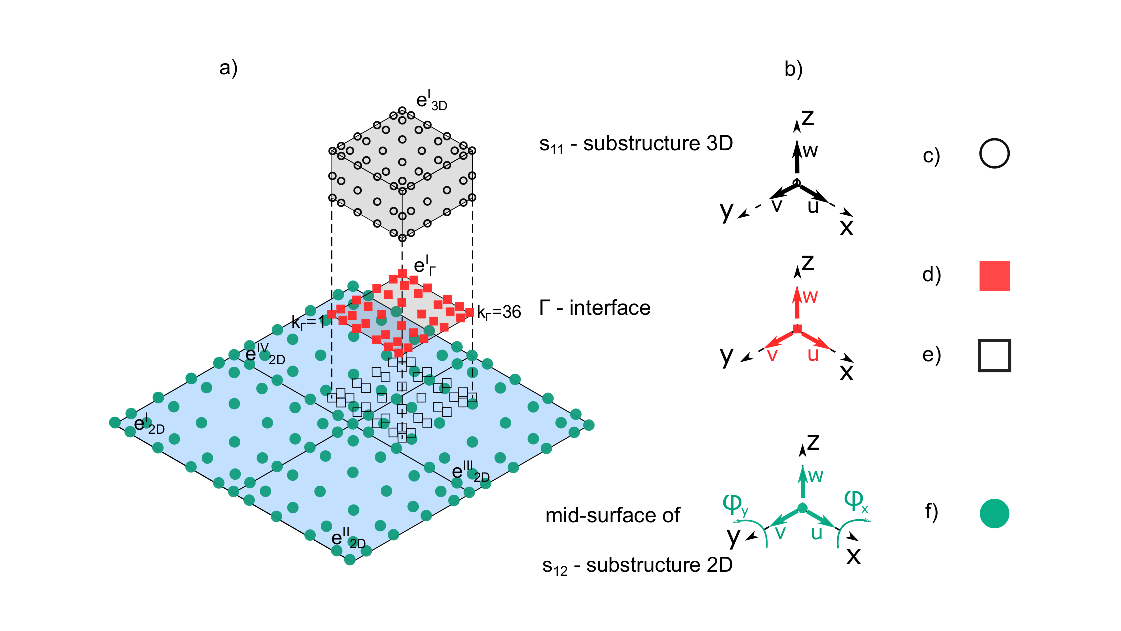
\includegraphics[width=1\linewidth]{../../figures/eps/interface_2D3D.eps}
	\end{center}
	\caption{Non-matching interface setup: a) interface coupling, b) degrees-of-freedom of the interface and the substructures, c) the nodes of the 3D substructure, d) interface nodes inherited from 3D substructure, e) interface nodes projection on the 2D substructure, f) the nodes of the 2D substructure}
	\label{fig:interface}
\end{figure}
where \(s_{i1}\) and \(s_{i2}\) are substructures connected by the interface \(\Gamma^i\). For the whole structure, the Eq.~\ref{eq:coupling} can be written in the matrix form:
\begin{eqnarray}
\textbf{G}\textbf{d}=\textbf{0}
\label{eq:cond_disp}
\end{eqnarray}
where \textbf{G} is the coupling matrix which contains the equations to interpolate the substructures displacements at the interfaces, and \(\textbf{d}\) is a global vector of displacements for \(nS\) number of substructures, composed as:
\begin{eqnarray}
\textbf{d} = \left\{\begin{array}{cccc}
\textbf{d}_1, & \textbf{d}_2, &\ldots, & \textbf{d}_{nS}
\end{array}\right\}^T
\label{eq:displacements}
\end{eqnarray}

\begin{algorithm}[H]
	\SetAlgoLined
	\KwResult{coupling matrix \textbf{G}}
	create empty \(nI \times nS\) cell array: \(\mathbf{G} = cell(nI,nS)\)\;
	\For{i = 1 \KwTo nI}{
		find two common structures of interface \(\Gamma^i\): \(s_i = 
		(s_{i1},s_{i2})\)\;
		\For{j = 1 \KwTo 2}{
			create \(n^{\Gamma^i}\times n^{s_{ij}}\) null matrix 
			\(\mathbf{G}^{s_{ij}}_i\),\\
			\For{k = 1 \KwTo \(n^{\Gamma^i}\)} {
				find \(ownerElement^{s_{ij}}_k\) in the structure \(s_{ij}\) 
				containing interface node \(k\) with global coordinates vector: 
				\(X_p=(x^k_p,y^k_p)\)\;
				assign vector \(X_e=(x_e,y_e)\) of coordinates of all nodes in 
				\(ownerElement^{s_{ij}}_k\)\;
				assign initial coordinates 
				\(X_{\kappa}=(x^k_{\kappa},y^k_{\kappa})\) to the nearest node 
				in 
				\(ownerElement^{s_{ij}}_k\) to node \(k\)\;
				transform global coordinates \(X_{\kappa}\) to a local coordinate system \(\xi_{\kappa}=\xi(X_{\kappa});\quad 
				\eta_{\kappa}=\eta(X_{\kappa})\)\;
				\While{\(\left|X_p-X_{\kappa}\right|>tol\)}{
					\(\xi_{\kappa+1}=\xi_{\kappa}+(J^{-1}_{\kappa})_{11}.*(x^k_p-x_{\kappa}^k)+(J^{-1}_{\kappa})_{12}.*(y^k_p-y_{\kappa}^k)\)\;
					\(\eta_{\kappa+1}=\eta_{\kappa}+(J^{-1}_{\kappa})_{21}.*(x^k_p-x_{\kappa}^k)+(J^{-1}_{\kappa})_{22}.*(y^k_p-y_{\kappa}^k)\)\;
					\(X_{\kappa}=N(\xi_{\kappa+1},\eta_{\kappa+1})X_e\)\;
				}
				\(\xi^k_p\approx \xi_{\kappa+1},\quad \eta^k_p\approx 
				\eta_{\kappa+1}\)\;
				\(\mathbf{G}^{s_{ij}}_i(k,nX_e)=N(\xi^k_p,\eta^k_p)\)\;
			}
			\uIf{elements of \(s_{ij}\) are 3D} {
				
				\(\mathbf{G}\{i,s_{ij}\}=\left[\begin{array}{ccc}
				\mathbf{G}^{s_{ij}}_i & \mathbf{0} & \mathbf{0}\\
				\mathbf{0} & \mathbf{G}^{s_{ij}}_i & \mathbf{0}\\
				\mathbf{0} & \mathbf{0} & \mathbf{G}^{s_{ij}}_i
				\end{array} \right]
				\)\;
			}
			\ElseIf{elements of \(s_{ij}\) are 2D} {
				
				\(\mathbf{G}\{i,s_{ij}\}=\left[\begin{array}{ccccc}
				\mathbf{G}^{s_{ij}}_i & \mathbf{0} & \mathbf{0} & 
				\frac{h_{ij}}{2}\mathbf{G}^{s_{ij}}_i & \mathbf{0}\\
				\mathbf{0} & \mathbf{G}^{s_{ij}}_i & \mathbf{0} & \mathbf{0} & 
				\frac{h_{ij}}{2}\mathbf{G}^{s_{ij}}_i\\
				\mathbf{0} & \mathbf{0} & \mathbf{G}^{s_{ij}}_i & \mathbf{0} & 
				\mathbf{0}
				\end{array} \right]
				\)\;	}
			
		}
	}
where \(nI\) and \(nS\) are numbers of the interfaces and the structures, respectively; \(n^{\Gamma^i}\) and \(n^{s_{ij}}\) are numbers of nodes of the interface \(i\), and the structure \(s_{ij}\), respectively; \(\eta^k_p\) and  \(\xi^k_p\) are local coordinates of \(X_p\), respectively; \(J_{\kappa}\) are Jacobians evaluated at \((\xi_{\kappa+1},\eta_{\kappa+1})\) and \(N(\xi_{\kappa+1},\eta_{\kappa+1})\) is the shape function evaluated at \((\xi_{\kappa+1},\eta_{\kappa+1})\), \(nX_e\) is the vector of global order numbers of all nodes in the \(Elements^{s_{ij}}_k\), \(h_{ij}\) is a thickness of the structure \(s_{ij}\) and \(tol\) is a termination criterion for iterations.
	\caption{Matrix G formulation}
	\label{alg:G_matrix}
\end{algorithm}
The general formulation of the matrix \textbf{G} is proposed in Algorithm \ref{alg:G_matrix}.
The main task of the algorithm is to calculate shape functions for each adjacent substructures at the points \(X_p=(x_p^k,y_p^k)\), which are projections of the interface nodes onto these substructures.
The shape function can be calculated after finding an owner element and local coordinates of the points.
Owner element is a spectral element in the domain of the substructure \(s_{ij}\) which contains interface node, for example, interface node \(k_\Gamma=36\) (see~Fig.~\ref{fig:interface}a)) is located in the element \(e^{I}_{3D}\) and \(e^{III}_{2D}\) for the substructures \(s_{11}\) and \(s_{12}\), respectively.
It can be found within two ways: using Matlab's built-in function \verb+inpolygon+ or more efficient procedure proposed by Silva et al. \cite{silva2009exact} which was used in the current implementation.
The transformation from global to local coordinates was realised by the iterative method presented in the work of Li et al.~\cite{li2014efficient}.

The computational effectiveness of Algorithm~\ref{alg:G_matrix} can be easily improved if certain precautions are taken.
Firstly, the mesh of the interface has to be based on the mesh from one of the substructures \(s_i1\), \(s_i2\), which may be referred to as a slave.
So, the shape function takes only the values of one and zeros.
Moreover, the code can be implemented in vectorized form rather than using a for-loops.

\subsection{Elementary governing equations of motion}
\label{sec:motion}
The classical equations of motion \(\textbf{M}\ddot{\textbf{d}} + \textbf{C}\dot{\textbf{d}} + \textbf{K}\textbf{d} = \textbf{F}\) known from FEM are complemented by piezoelectric and interface coupling. Thus, the governing equations are defined as:
\begin{eqnarray}
\textbf{M}_{dd} \widehat{\ddot{\textbf{d}}} + \textbf{C}_{dd} \widehat{\dot{\textbf{d}}} + \textbf{K}_{dd} \widehat{\textbf{d}} + \textbf{K}_{d\phi} \widehat{\boldsymbol{\phi}} = \textbf{F} - \textbf{G}^T \boldsymbol{\lambda},
\label{eq:motion}
\end{eqnarray}
\begin{eqnarray}
\textbf{K}_{\phi d}\widehat{\textbf{d}} + \textbf{K}_{\phi \phi} \widehat{\boldsymbol{\phi}} = \textbf{Q}
\label{eq:piezocoupling}
\end{eqnarray} 

where \(\textbf{M}_{dd}\), \(\textbf{C}_{dd}\), \(\textbf{K}_{dd}\) are structural mass, damping and stiffness matrices, respectively; \(\textbf{K}_{\phi d}={\textbf{K}_{d\phi}}^T\) are piezoelectric coupling matrices; \(\textbf{K}_{\phi \phi}\) is the dielectric permittivity matrix, \(\widehat{\textbf{d}}\) is the vector of unknown nodal displacements, and \(\widehat{\boldsymbol{\phi}}\) is the electric potential vector; \(\textbf{F}\) the nodal external force vector, \(\textbf{Q}\) is the nodal charge vector, \(\boldsymbol{\lambda}\) is the Lagrange multipliers vector, and \(\textbf{G}\) is the interface coupling matrix; \((\dot{\ })=\frac{\partial}{\partial t}\).
The formulae of the matrices are provided in App.~\ref{app:matrices}.
The coupling is realised by imposing the traction forces, represented by a vector of Lagrange multipliers. 

\subsection{Transformation of the core elements}
\label{sec:transformation}
All core elements are rotated relative to both skins, so it is necessary to transform degrees of freedom from the local core's coordinate system to the global system.
For this purpose, an additional sixth global dof has been incorporated, i.e. rotation with respect to the z-axis.
Firstly, a part of the mass matrix accounted for rotary inertia (see App. \ref{app:matrices}) is globalised as follows:
\begin{eqnarray}
\textbf{M}_R^g=\textbf{a}\,\textbf{M}_R^l\,\textbf{a}^{-1}
\label{eq:inertia}
\end{eqnarray}
where \(\textbf{a}\) is general rotation matrix obtained from the multiplication of basic rotation matrices, and for the regular hexagonal core a is equal to:
\begin{eqnarray}
\textbf{a}=\left [ 
\begin{array}{ccc}
m & -n & 0\\
0 & 0 & -1\\
n & m & 0\\
\end{array}
\right ]
\label{eq:rotation}
\end{eqnarray}
where \(m=\cos(\alpha),\:n=\sin(\alpha)\), for \(\alpha\in{[0^\circ,\,60^\circ,\,120^\circ,180^\circ,\,240^\circ,\,300^\circ]}\) depending on which wall of the cell it is applied to.

The stiffness--strain relationship in local and global coordinate systems is given by:
\begin{eqnarray}
\begin{array}{ccc}
\left [
\begin{array}{c}
\sigma^l_{11}\\
\sigma^l_{22}\\ 
\sigma^l_{33}\\ 
\sigma^l_{23}\\
\sigma^l_{13}\\
\sigma^l_{12}\\
\end{array}
\right ]=
\textbf{c}\,\left [
\begin{array}{c}
\epsilon^l_{11}\\
\epsilon^l_{22}\\ 
\epsilon^l_{33}\\
\gamma^l_{23}\\
\gamma^l_{13}\\
\gamma^l_{12}\\
\end{array}
\right ], & and &
\left [
\begin{array}{c}
\sigma^g_{11}\\
\sigma^g_{22}\\ 
\sigma^g_{33}\\ 
\sigma^g_{23}\\
\sigma^g_{13}\\
\sigma^g_{12}\\
\end{array}
\right ]=
\bar{\textbf{c}}\,\left [
\begin{array}{c}
\epsilon^g_{11}\\
\epsilon^g_{22}\\ 
\epsilon^g_{33}\\
\gamma^g_{23}\\
\gamma^g_{13}\\
\gamma^g_{12}\\
\end{array}
\right ]
\end{array}
\label{eq:stress_global}
\end{eqnarray}
The global form of the stiffness matrix \(K\), involves the determination of stiffness tensor \(\bar{c}\) from Eq.~\ref{eq:stress_global}.
The transformation of the stress tensor is expressed as:
\begin{eqnarray}
\left [ 
\begin{array}{ccc}
\sigma^g_{11} & \sigma^g_{12} & \sigma^g_{13}\\
\sigma^g_{21} & \sigma^g_{22} & \sigma^g_{23}\\
\sigma^g_{31} & \sigma^g_{32} & \sigma^g_{33}\\
\end{array}
\right ]
=
\textbf{a}\,
\left [ 
\begin{array}{ccc}
\sigma^l_{11} & \sigma^l_{12} & \sigma^l_{13}\\
\sigma^l_{21} & \sigma^l_{22} & \sigma^l_{23}\\
\sigma^l_{31} & \sigma^l_{32} & \sigma^l_{33}\\
\end{array}
\right ]
\,\textbf{a}^T
\label{eq:sigma_tensor}
\end{eqnarray}
After the multiplication of matrices and using the symmetry of the stress tensor Eq.~\ref{eq:sigma_tensor} can be rewritten in a simplified form:

\begin{eqnarray}
\left [
\begin{array}{c}
\sigma^g_{11}\\
\sigma^g_{22}\\ 
\sigma^g_{33}\\ 
\sigma^g_{23}\\
\sigma^g_{13}\\
\sigma^g_{12}\\
\end{array}
\right ]=
\textbf{T}\,\left [
\begin{array}{c}
\sigma^l_{11}\\
\sigma^l_{22}\\ 
\sigma^l_{33}\\
\sigma^l_{23}\\
\sigma^l_{13}\\
\sigma^l_{12}\\
\end{array}
\right ]
\label{eq:stress}
\end{eqnarray}

Analogously, a strain relationship also is given in the form:
\begin{eqnarray}
\begin{array}{ccc}
\left [
\begin{array}{c}
\epsilon^g_{11}\\
\epsilon^g_{22}\\ 
\epsilon^g_{33}\\ 
\epsilon^g_{23}\\
\epsilon^g_{13}\\
\epsilon^g_{12}\\
\end{array}
\right ]=
\textbf{T}\,\left [
\begin{array}{c}
\epsilon^l_{11}\\
\epsilon^l_{22}\\ 
\epsilon^l_{33}\\
\epsilon^l_{23}\\
\epsilon^l_{13}\\
\epsilon^l_{12}\\
\end{array}
\right ], & and & \left [
\begin{array}{c}
\epsilon_{11}\\
\epsilon_{22}\\ 
\epsilon_{33}\\ 
\gamma_{23}\\
\gamma_{13}\\
\gamma_{12}\\
\end{array}
\right ]=
\textbf{R}\,\left [
\begin{array}{c}
\epsilon_{11}\\
\epsilon_{22}\\ 
\epsilon_{33}\\
\epsilon_{23}\\
\epsilon_{13}\\
\epsilon_{12}\\
\end{array}
\right ]
\end{array}
\label{eq:strain}
\end{eqnarray}
where \(\textbf{R}\) is the Reuter's matrix, defined as:
\begin{eqnarray}
\textbf{R} = \left [
\begin{array}{cccccc}
1 & 0 & 0 & 0 & 0 & 0\\
0 & 1 & 0 & 0 & 0 & 0\\
0 & 0  & 1 & 0 & 0 & 0\\
0 & 0 & 0 & 2 & 0 & 0\\
0 & 0 & 0 & 0 & 2 & 0\\
0 & 0 & 0 & 0 & 0 & 2
\end{array}
\right ]
\label{eq:reuters}
\end{eqnarray}
Using the Eqs.~\ref{eq:rotation} through \ref{eq:reuters}, the relationship of stress--strain in the global frame can be expressed as:
\begin{eqnarray}
\left [
\begin{array}{c}
\sigma^g_{11}\\
\sigma^g_{22}\\ 
\sigma^g_{33}\\ 
\sigma^g_{23}\\
\sigma^g_{13}\\
\sigma^g_{12}\\
\end{array}
\right ]=
\textbf{T}\,\textbf{c}\,\textbf{R}\,\textbf{T}^{-1}\,\textbf{R}^{-1}\,
\left [
\begin{array}{c}
\epsilon^g_{11}\\
\epsilon^g_{22}\\ 
\epsilon^g_{33}\\
\gamma^g_{23}\\
\gamma^g_{13}\\
\gamma^g_{12}\\
\end{array}
\right ]
\label{eq:stress-strain}
\end{eqnarray}
Therefore, transformed stiffness tensor for the core's elements is equal:
\begin{eqnarray}
\bar{\textbf{c}}=\textbf{T}\,\textbf{c}\,\textbf{R}\,\textbf{T}^{-1}\,\textbf{R}^{-1}
\label{eq:c_global}
\end{eqnarray}
\subsection{A solution of the equation of motion}
\label{sec:time_integration}
Assuming \(\textbf{b}\) and \(\textbf{f}\) represent order lists of the electrodes nodes and free nodes of the PZT, respectively, the electrical potential vector is rewritten:
\begin{eqnarray}
\widehat{\boldsymbol{\phi}} = \left \{\begin{array}{cc}
\widehat{\boldsymbol{\phi}}(\textbf{b}) &
\widehat{\boldsymbol{\phi}}(\textbf{f})
\end{array}\right \}^T
\label{eq:potential}
\end{eqnarray}
Then, Eq. \ref{eq:piezocoupling} is expressed as:
\begin{eqnarray}
\left [\begin{array}{c}
\textbf{K}_{\phi d}(\textbf{b},:) \\
\textbf{K}_{\phi d}(\textbf{f},:)
\end{array}\right]
\left \{\widehat{\textbf{d}}\right\} +
\left [\begin{array}{cc}
\textbf{K}_{\phi \phi}(\textbf{b},\textbf{b}) & \textbf{K}_{\phi \phi}(\textbf{b},\textbf{f})\\
\textbf{K}_{\phi \phi}(\textbf{f},\textbf{b}) & \textbf{K}_{\phi \phi}(\textbf{f},\textbf{f})
\end{array}\right]
\left \{\begin{array}{c}
\widehat{\boldsymbol{\phi}}(\textbf{b}) \\
\widehat{\boldsymbol{\phi}}(\textbf{f})
\end{array}\right \} = 
\left \{\begin{array}{c}
\textbf{Q} \\
\textbf{0}
\end{array}\right \}
\label{eq:piezoboundary}
\end{eqnarray} 
where the notation \(\textbf{K}(\textbf{row},\textbf{col})\) uses vectors \(\textbf{row}\) and \(\textbf{col}\) to extract rows and columns from the matrix \(\textbf{K}\), respectively, and \((:)\) means all rows or columns of \(\textbf{K}\).
The electrical potential of the free nodes can be extracted from Eq. \ref{eq:piezoboundary}:
\begin{eqnarray}
\widehat{\boldsymbol{\phi}}(\textbf{f}) = -\textbf{K}_{\phi\phi}^{-1}(\textbf{f},\textbf{f})\left[\textbf{K}_{\phi d}(\textbf{f},:) \widehat{\textbf{d}} + \textbf{K}_{\phi\phi}(\textbf{f},\textbf{b})\widehat{\boldsymbol{\phi}}(\textbf{b}) \right]
\label{eq:freePotetial}
\end{eqnarray}
Substituting Eq. \ref{eq:potential} and \ref{eq:freePotetial} into Eq. \ref{eq:motion}, the equation of motion can be rearranged into the form:
\begin{eqnarray}
\textbf{M}_{dd} \widehat{\ddot{\textbf{d}}} + \textbf{C}_{dd} \widehat{\dot{\textbf{d}}} + (\textbf{K}_{dd}-\textbf{K}_{s}) \widehat{\textbf{d}}  = \textbf{F} + \textbf{K}_{a} \widehat{\boldsymbol{\phi}}(b) - \textbf{G}^T \boldsymbol{\lambda},
\label{eq:motionD}
\end{eqnarray}
where  \(\textbf{K}_a=\textbf{K}_{d\phi}(:,f)\textbf{K}_{\phi \phi}^{-1}(f,f)\textbf{K}_{\phi \phi}(\textbf{f},\textbf{b})-\textbf{K}_{d\phi}(:,\textbf{b})\), \(\textbf{K}_s=\textbf{K}_{d \phi}(:,\textbf{f})\textbf{K}_{\phi \phi}^{-1}(\textbf{f},\textbf{f})\textbf{K}_{\phi d}(\textbf{f},:)\).
The unknown vector of displacements \(\widehat{\textbf{d}}_t\) is found using a central difference algorithm \cite{kudela20093d}.
Thus, Eq.~(\ref{eq:motionD}) is rewritten as:
\begin{eqnarray}
\left(\frac{1}{\Delta t^2}\textbf{M}_{dd}+\frac{1}{2\Delta t}\textbf{C}_{dd} \right)\widehat{\textbf{d}}_{t+\Delta t}=
\textbf{F}_t+\textbf{K}_a\widehat{\boldsymbol{\phi}}_t(b)-\left( \textbf{K}_{dd}-\textbf{K}_s\right)\widehat{\textbf{d}}_t\nonumber\\
+\frac{2}{\Delta t^2}\textbf{M}_{dd}\widehat{\textbf{d}}_t-\left(\frac{1}{\Delta t^2}\textbf{M}_{dd}-\frac{1}{2\Delta t}\textbf{C}_{dd}\right)\widehat{\textbf{d}}_{t-\Delta t}-\textbf{G}^T\boldsymbol{\lambda}_t
\label{eq:CDE}
\end{eqnarray}
where \(\Delta t\) is the time increment.

Imposing the constrain Eq. \ref{eq:cond_disp}, the vector of Lagrange multipliers \(\boldsymbol{\lambda}_t\) can be extracted from Eq. \ref{eq:CDE}:\begin{eqnarray}
\boldsymbol{\lambda}_t = {\left(\textbf{G}\textbf{L}_+^{-1}\textbf{G}^T \right)}^{-1}\textbf{G}\textbf{L}_+^{-1} \Bigg[ \textbf{F}_t+\textbf{K}_a\widehat{\boldsymbol{\phi}}_t(b)+\left.\left(\frac{2}{\Delta t^2}\textbf{M}_{dd}-\textbf{K}_{dd}+\textbf{K}_s\right)\widehat{\textbf{d}}_t -\textbf{L}_-\widehat{\textbf{d}}_{t-\Delta t} \right]
\label{eq:lambda}
\end{eqnarray}
where \(\textbf{L}_{\pm}=\frac{1}{\Delta t^2}\textbf{M}_{dd}\pm\frac{1}{2\Delta t}\textbf{C}_{dd}\).

\section{Numerical simulations}
\label{sec:numerical}
\subsection{Sample configuration}
\label{sec:sample}
The sample consists of aluminium honeycomb attached between two carbon fibre reinforced polymer (CFRP) plates by the adhesive layers (Fig.~\ref{fig:honeycomb}a)).
Material properties used in the simulations are gathered in App.~\ref{app:properties}.
One pair of circular PZT transducers were mounted on the top skin to generate and receive GW signals.
A glue layer under transducers was not considered.

The adhesive layer elements from a circular area of damage were removed from the model to simulate disbonds in the HSC, as it was implemented by Cerniglia et al. \cite{cerniglia20103d}.
The failure was placed in the structure centre, between the top skin and the core. 
This model is simple for implementation and does not affect the convergence of the time integration algorithm.
However, it does not take into account the contact between the structures, so the nodes of particular elements in this area may interpenetrate.
The size of disbonds was the subject of the parametric study aiming at finding the damage effect on GW propagation.

The following dimensions and parameters were assumed:
\begin{itemize}
	\item CFRP skins --- L = 500, W = 314, H = 1 mm, fibers volume fraction 
	50\%, stacking sequence 
	\([0^\circ,90^\circ,0^\circ,90^\circ,0^\circ,90^\circ,0^\circ,90^\circ]\),
	\item Core --- \(\Phi\) = 19, h = 10, w = 0.07 mm 
	(Fig.~\ref{fig:honeycomb}b)),
	\item Adhesive --- L = 500, W = 314, H = 0.5 mm,
	\item PZT --- \(\Phi\) = 10, h = 0.5 mm, location \#1 \((x_1,y_1)=(-80,0)\) 
	mm,	\#2 \((x_2,y_2)=(80,0)\) mm,
	\item Disbonds \(\Phi = \left [0, 20, 40, 60, 80, 100, 120 \right ]\).
\end{itemize}

\begin{figure}
	\begin{center}
		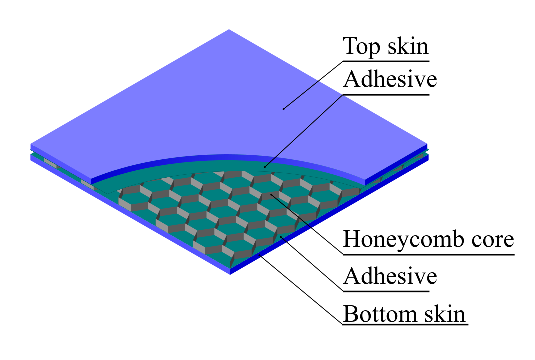
\includegraphics[width=1\linewidth]{../../figures/eps/honeycomb.eps}
	\end{center}
	\caption{Sample configuration: a) top view of the sample, b) honeycomb sandwich substructures, c) detail of the honeycomb cell}
	\label{fig:honeycomb}
\end{figure}

\subsection{Simulation parameters}
\label{sec:simulation}
The inversion of the matrix \(\left [\textbf{GL}_+^{-1}\textbf{G}^T\right ]\) is necessary to calculate the vector of Lagrange multipliers in Eq. \ref{eq:lambda}).
While \(\textbf{L}_+\) is a diagonal matrix, the sparsity of the matrix \(\textbf{G}\) has a significant influence on the computation cost. .
Therefore, during the generation of the mesh, the following steps were taken to reduce the number of non-zero matrix values in the matrix \(\textbf{G}\).

One spectral element was intended for each wall of the honeycomb core, while the meshes of the skin plates and the adhesive layers were divided by three rhombus elements per area under the core cell.
In this way, the interface nodes coincide with the nodes lying on the hexagon edges (thick line on Fig. \ref{fig:skin_mesh} b)).
In the case of PZT transducers, the mesh was generated by using external GMSH software \cite{geuzaine2009gmsh} (see Fig.~\ref{fig:skin_mesh} c)).
To achieve at least six nodes per wavelength within the assumed excitation range, 2D and 3D elements consist of \(4 \times 4\) and \(4 \times 4 \times 4\) nodes, respectively. 

\begin{figure}
	\begin{center}
		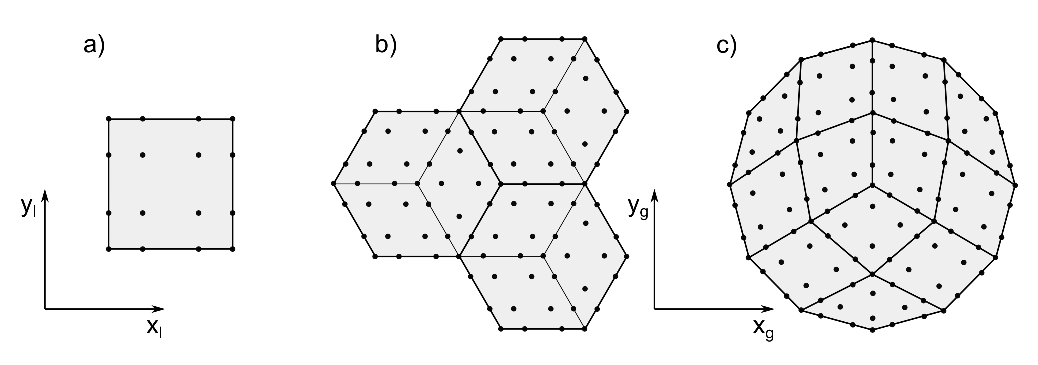
\includegraphics[width=1\linewidth]{../../figures/eps/skin_mesh.eps}
	\end{center}
	\caption{The mesh with the nodes distribution, a) spectral element of the core's wall, b) excerpt of the skin plate, c) top view of the PZT transducer mesh}
	\label{fig:skin_mesh}
\end{figure}
\begin{figure}
	\begin{center}
		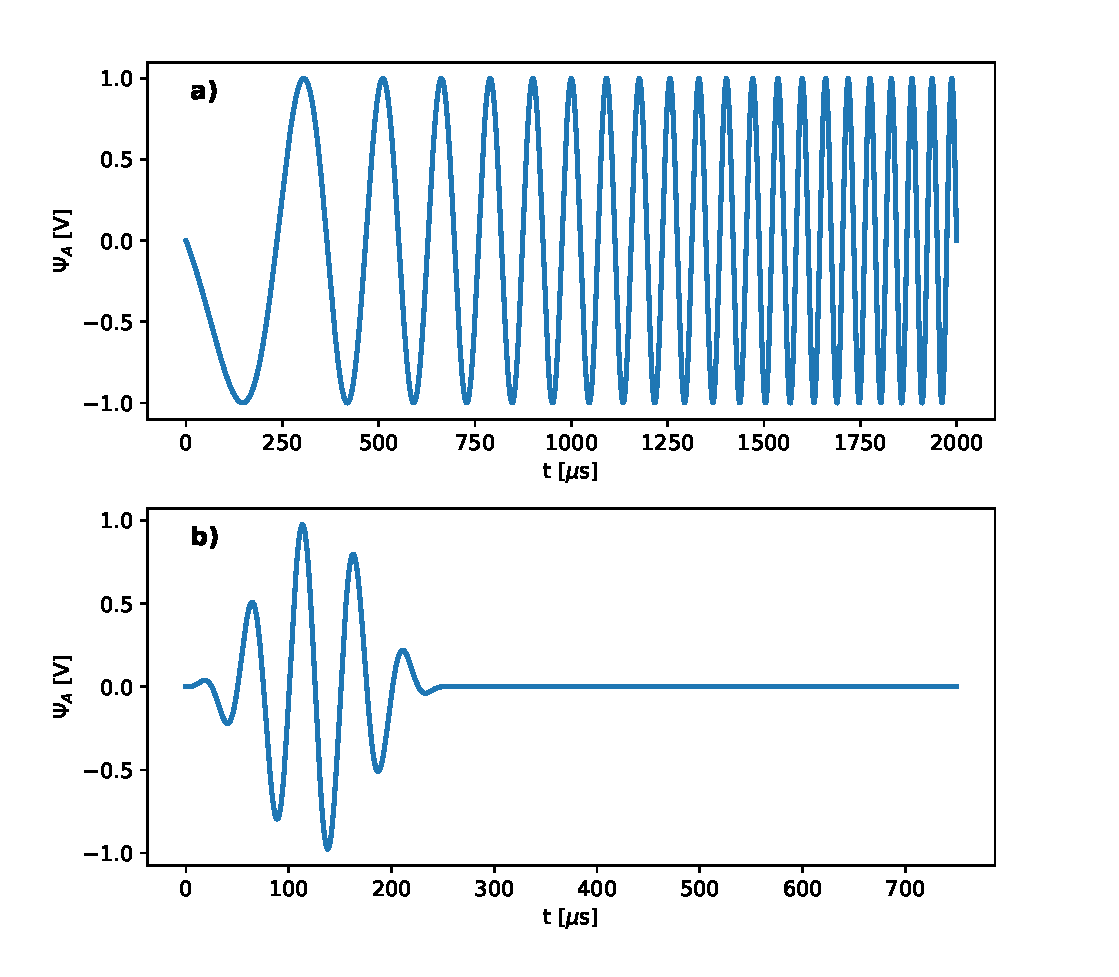
\includegraphics[width=1\linewidth]{../../figures/eps/signal.eps}
	\end{center}
	\caption{Excitation signal, a) chirp in a range of 0--20 kHz, b) five-cycle sine pulse with central frequency 20 kHz}
	\label{fig:signal}
\end{figure}

The analysis was conducted with a wide bandwidth chirp signal in the range of 0--20 kHz (Fig.~\ref{fig:signal}a).
Total calculation time was set to 2 ms with the time increment \(\Delta t=10\) ns.

\subsection{Homogenised model}
\label{sec:homogenization}
In the paper, comparative studies were carried out between the current model and the homogenised one. 
In the homogenised model, the values of material constants of the panel core were calculated according to the method presented by Malek and Gibson \cite{malek2015effective}.
The orthotropic mechanical properties for aluminium core are gathered in Table \ref{tab:properties_eff}, while the properties for other structures, i.e. skins, adhesive layers and sensors remained unchanged.
To the comparison, a narrowband excitation signal was chosen in the form of five-cycles sine pulse in a Hanning window (Fig.~\ref{fig:signal}b). The central frequency was set to 20 kHz, which is the maximum frequency of the chirp signal from Fig.~\ref{fig:signal}a).

\section{Results}
\label{sec:results}
\subsection{Comparison of the models}
The advantage of the present model in comparison to the homogenised one can be immediately pointed out by analysis of the propagating wavefield (see Fig. \ref{fig:wavefield}).
The wavefield of the proposed model is much more realistic.
It reveals wave entrapment in the honeycomb cells.
Such an effect is not present in the homogenised model.
It also causes, that S0 to A0 mode conversion at sensor location is much more visible in the homogenised model (Fig.~\ref{fig:wavefield} left) than in the proposed model (Fig. \ref{fig:wavefield} right).

It can be noticed in Fig.~\ref{fig:wavefield}) that the wave propagates in a manner typical for orthotropic material in case of both models, i.e. the wave velocity depends on the angle of propagation.
In addition to the material properties of skins, velocity profiles highly depend on the core properties.
This behaviour can be observed for both models.
The highest velocities of A0 and S0 mode are observed in $0^{\circ}$ direction, while the minimum values are for $45^{\circ}$ (see. Fig.~\ref{fig:speed}).
The A0 mode velocities are significantly lower in the current model than in the homogenised one.
The differences are in a range from 12 to 29\%, and only up to 3\% for S0 mode.  

In Fig.~\ref{fig:velocity} d) one can also notice differences in the particles velocity amplitude after the pulse has passed.
For that period, the amplitude of particle velocity \(V_z\) is 2.8 times higher for the present model, due to reflections of the wave within the core walls.

\label{comparison}
\begin{figure}
	\begin{center}
		\includegraphics[width=1\linewidth]{../../figures/eps/wavefield_1.eps}
	\end{center}
	\caption{Full wavefield of the guided waves propagating in the sandwich for the present model and the homogenised one}
	\label{fig:wavefield}
\end{figure}
\begin{figure}
	\begin{center}
		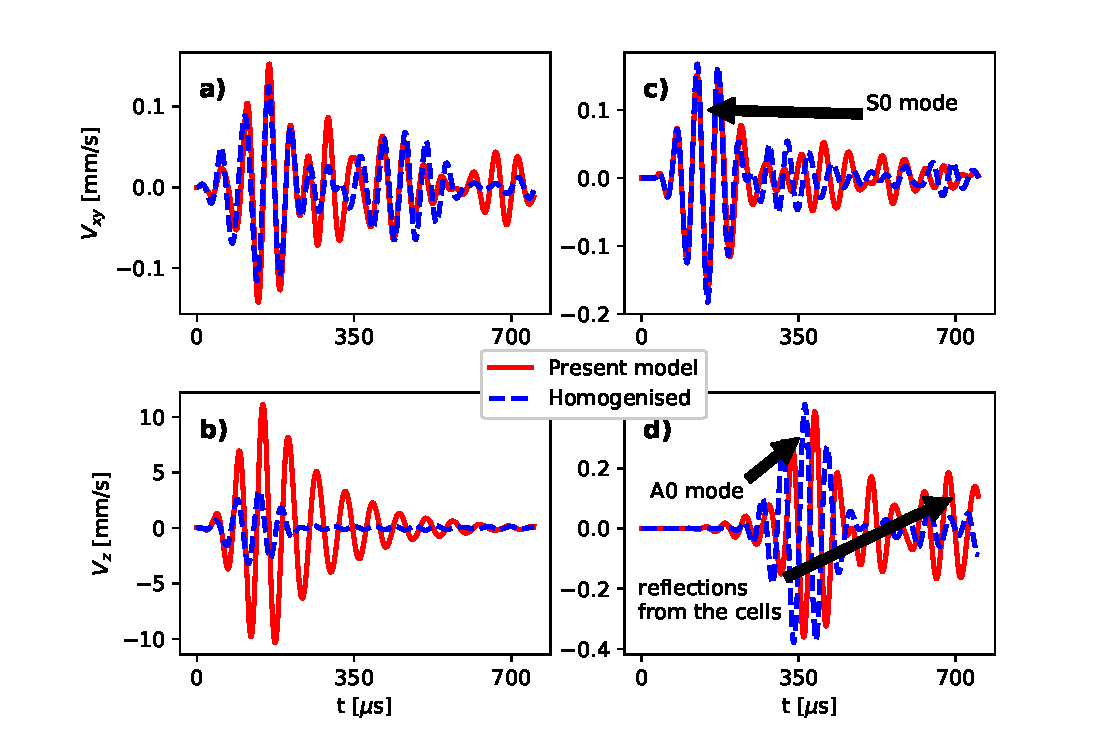
\includegraphics[width=1\linewidth]{../../figures/eps/velocity.eps}
	\end{center}
	\caption{Particle velocity at point: a, b) P0(-86,0) mm, and c, d) P1(114,0) mm}
	\label{fig:velocity}
\end{figure}
\begin{figure}
	\begin{center}
		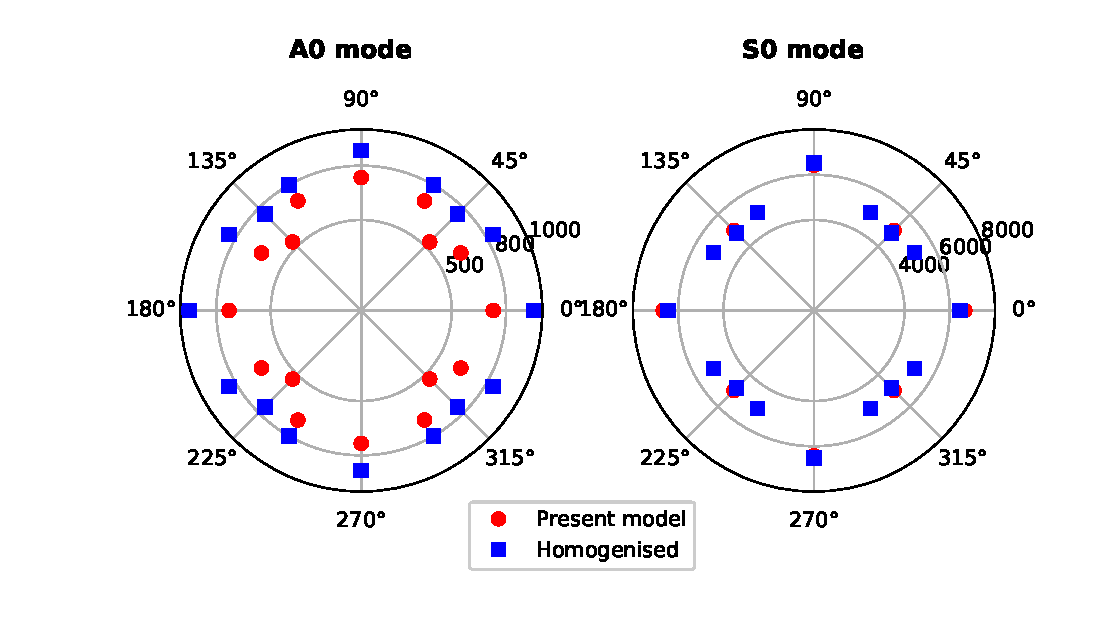
\includegraphics[width=1\linewidth]{../../figures/eps/cg.eps}
	\end{center}
	\caption{Group velocity in the function of propagation angle}
	\label{fig:speed}
\end{figure}

Therefore, differences in values recorded by the sensor are expected, as shown in Fig. \ref{fig:voltage}.

\begin{figure}
	\begin{center}
		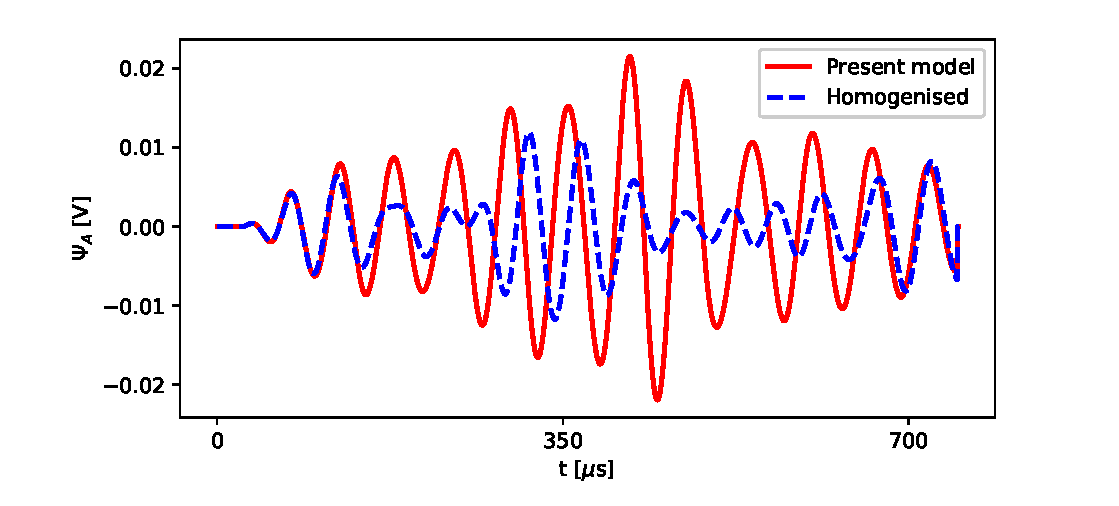
\includegraphics[width=1\linewidth]{../../figures/eps/voltage.eps}
	\end{center}
	\caption{Comparison of the voltage response of the sensors}
	\label{fig:voltage}
\end{figure}

\subsection{Model-Assisted Damage Identification Function}
\label{MADIF}

The transmission coefficient of elastic waves decreases locally within the defect area because the acoustic impedance of air is less than that of the adhesive layer.
As a result, the amplitude of the transmitted wave varies depending on the damage size.
\begin{figure}
	\begin{center}
		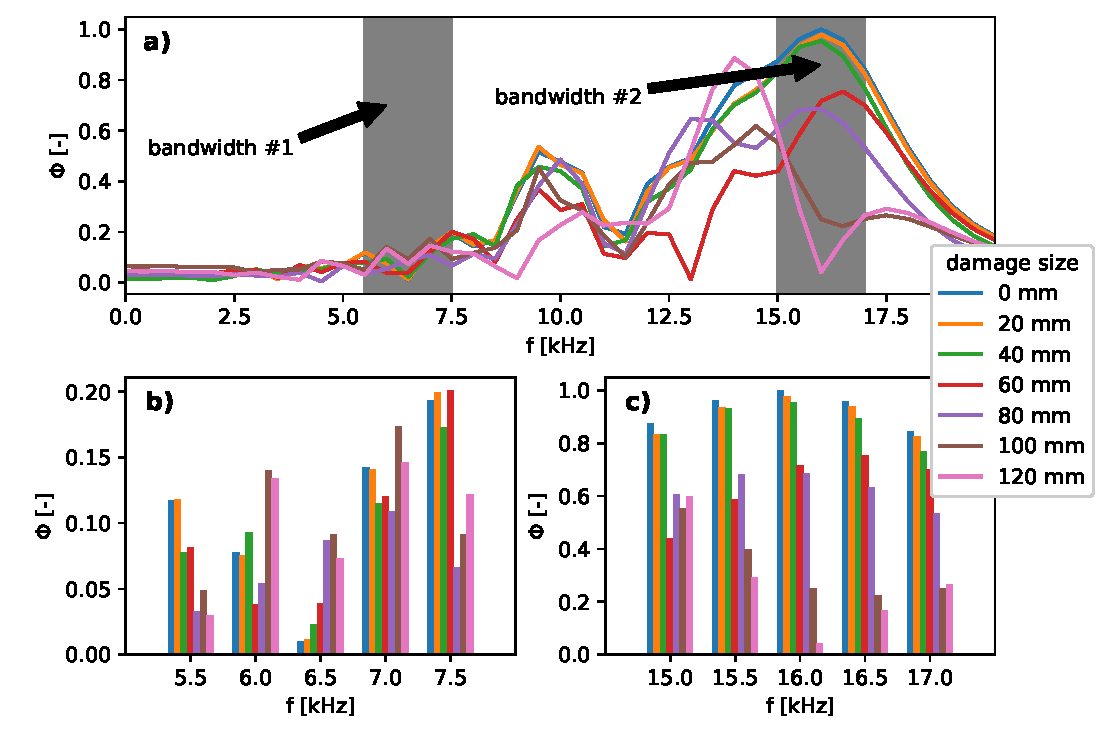
\includegraphics[width=1\linewidth]{../../figures/eps/mgntPhiFFT.eps}
	\end{center}
	\caption{The sensor signal in frequency domain a) full excitation bandwidth, b) bandwidth \#1, c) bandwidth \#2}
	\label{fig:signals}
\end{figure}
\begin{figure}
	\begin{center}
		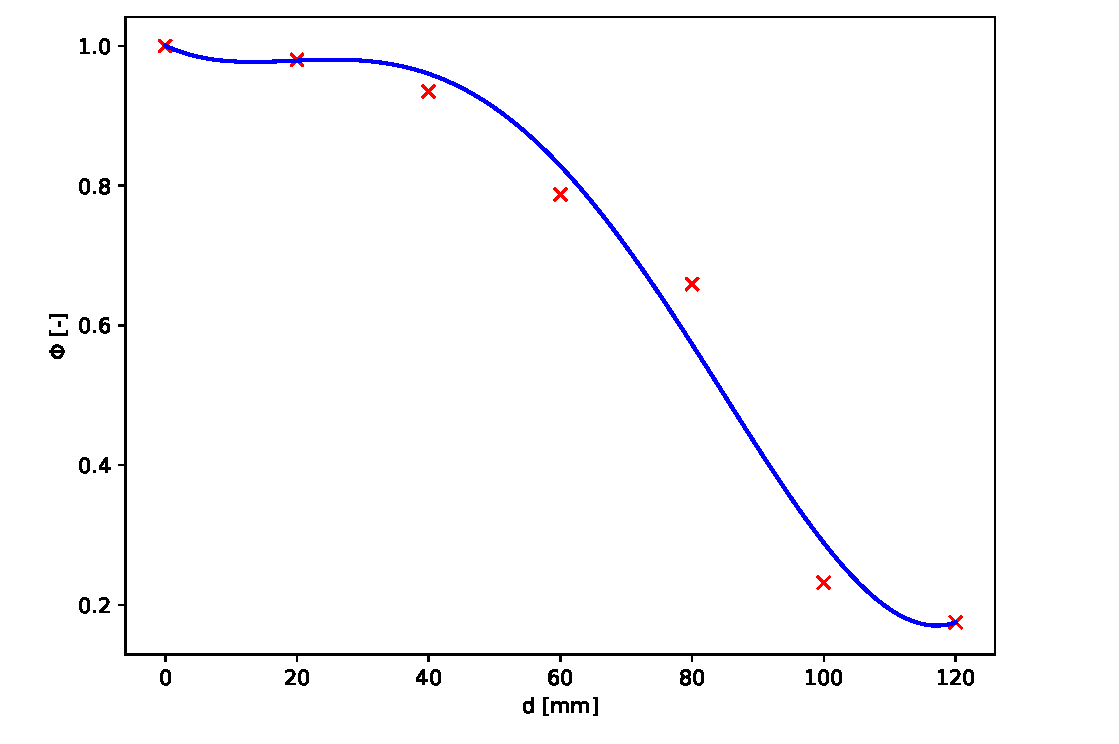
\includegraphics[width=1\linewidth]{../../figures/eps/madif.eps}
	\end{center}
	\caption{The Model-Assisted Damage Identification Function (MADIF) for 16.5 kHz}
	\label{fig:madif}
\end{figure}
To determine the effect of the damage size on GW propagation, the signal obtained by the sensor was taken into account.
The signal represents an average value of the electrical potential of the nodes belonging to the upper layer of the sensor, calculated in each time step for different damage diameter.
For further analysis, the time domain characteristics were transformed to the frequency domain by the discrete Fourier transform, \(\Psi_S(f)=DFT(\Psi_S(t))\).
It can be noticed in Fig. \ref{fig:signals}a) that the signal amplitudes do not always decrease with increasing the diameter of the damage.
Therefore, to determine the MADIF, the frequency \(f_i\) was chosen from among the full excitation range for which the function is monotonous. Thus, the MADIF is defined as:
\begin{eqnarray}
I = \Psi_S(f_i,d)
\end{eqnarray}

This assumption is fulfilled by the frequency \(f_1=16.0\) and \(f_2=16.5\) kHz (Fig. \ref{fig:signals}c)).
The MADIF (blue, solid line on Fig. \ref{fig:madif}) was approximated by the polynomial interpolation of the amplitudes in the frequency 16.5 kHz (red, x marks on Fig. \ref{fig:madif}) obtained in the simulations. 

Normalized values of the MADIF are within a wide range, i.e. 0.2–1.0, which has a positive impact on the accuracy of the severity of damage indication.
This function can be used to identify damage to the physical sample associated with the model.
The severity of the failure is indicated on the determined characteristic for the sensor voltage value, measured under the simulation scheme.

\section{Conclusions}
\label{sec:conc}
This paper presents preliminary research on the possibility of using a model-assisted approach to identify the severity of damage in a composite structure using GW propagation.
For this purpose, the HSC panel model has been implemented with the actual geometry of the honeycomb core.
In contrast to  full structure homogenisation, which is the most common HSC model found in the literature, the interaction of the propagating wave with core cell walls is visible in the current model.
Moreover, the model is computationally efficient due to the use of SEM and 2D elements.
The present model has 25 times less number of DOF than a full 3D model (according to \cite{kudela2016parallel}, estimated no of DOF is twelve million) and only 1.2 more than the homogenised model.

In the future works, the model will be adapted to parallel calculations using a multi-core graphics card, which will further reduce solution time. Experimental research will also be conducted to test the proposed method on physical samples.

\funding{The research was funded by the Polish National Science Center under grant agreement no 2018/31/N/ST8/02865 and 2018/31/B/ST8/00454.}
\acknowledgments{"Authors are also grateful to Task-CI for allowing the use of Matlab and Parallel Computing Toolbox licences}
\conflictsofinterest{The authors declare no conflict of interest.}
%%%%%%%%%%%%%%%%%%%%%%%%%%%%%%%%%%%%%%%%%%
%% optional
\appendixtitles{no} %Leave argument "no" if all appendix headings stay EMPTY (then no dot is printed after "Appendix A"). If the appendix sections contain a heading then change the argument to "yes".
\appendix
\section{}
\label{app:matrices}
The formulae of matrices for 3D elements are:
\begin{eqnarray}
\textbf{M}_{dd}^e & = & \int_{V_e}\textbf{N}^T\rho \textbf{N} dV_e\\
\textbf{K}_{dd}^e & = & \int_{V_e}{\textbf{B}_d^e}^T\textbf{c}\textbf{B}_d^edV_e
\end{eqnarray}
where \textbf{c} is the stiffness tensor, \(\rho\) is mass density, and \(V_e\) is the element volume.

In the case of the 2D elements, matrices are defined as:
\begin{eqnarray}
\textbf{M}_{dd}^e & = &
\left [
\begin{array}{cc}
\textbf{M}_T^e & 0\\
0 & \textbf{M}_R^e
\end{array}
\right] =
\int_{\Omega_e}\textbf{N}^T\rho 
\left [
\begin{array}{cccccc}
h &  & &  &  &\\
0 & h & & & &\\
0 & 0 & h & & & \\
0 & 0 & 0 & \frac{h^3}{12} & &\\
0 & 0 & 0 & 0 & \frac{h^3}{12} &\\
0 & 0 & 0 & 0 & 0 & 0
\end{array} \right]
\textbf{N} d\Omega_e\\
\textbf{K}_{dd}^e & = & \int_{\Omega_e}{\textbf{B}_b^e}^T
\left[
\begin{array}{cc}
\textbf{A} & \textbf{B}\\
\textbf{B} & \textbf{D}
\end{array} \right]
\textbf{B}_b^ed \Omega_e+\int_{\Omega_e}{\textbf{B}_s^e}^T\hat{\textbf{A}}\textbf{B}_s^ed \Omega_e
\end{eqnarray}
where \(h=h_t+h_b\) is the element thickness, while \(h_{t(b)}\) is the distance between mid-plane and top(bottom) surface of the element, and \(\Omega_e\) is the element area:
\begin{eqnarray}
\textbf{A} & = & \textbf{c}_{ij}\,(h_t-h_b)\qquad i,j=1,2,6\nonumber\\
\textbf{B} & = & 1/2\, \textbf{c}_{ij}\,(h_t^2-h_b^2)\qquad i,j=1,2,6\nonumber\\
\textbf{D} & = & 1/3\, \textbf{c}_{ij}\,(h_t^3-h_b^3)\qquad i,j=1,2,6\nonumber\\
\hat{\textbf{A}} & = & 5/4\, \textbf{c}_{ij}\,\left[h_t-h_b-4/3\left(h_t^3-h_b^3\right)/h^2\right]\qquad i,j=4,5
\end{eqnarray}
The dielectric conductivity matrix \(\textbf{K}_{\phi \phi}^e\) and piezoelectric coupling matrix \(\textbf{K}_{u \phi}^e\) are defined:
\begin{eqnarray}
\textbf{K}_{d\phi}^e & = & \int_{V_e}{\textbf{B}_d^e}^T\textbf{e}^T \textbf{B}_{\phi}^ed V_e\\
\textbf{K}_{\phi \phi}^e & = & -\int_{V_e}{\textbf{B}_{\phi}^e}^T 
{\textbf{\(\epsilon\)}^S}^T \textbf{B}_{\phi}^edV_e
\end{eqnarray}

\section{}
\label{app:properties}
The mechanical properties of materials used in the simulations are gathered in Table~\ref{tab:properties}, and effective elastic properties for a single layer of unidirectional CRFP are presented in Table~\ref{tab:properties_eff}.
\begin{table}
	\centering
	\caption{\label{tab:properties}The mechanical properties of materials}
	\begin{tabular}{ccccc}\hline
		Material & \(E_{11}\) &  \(E_{33}\) & \(\nu_{12}\) & \(\rho\) \\
		& [GPa] &  [GPa] & [-] & [\(kg/m^3\)]\\
		\hline
		Carbon & 275.6 & 27.6 & 0.2 & 1900\\
		Epoxy & 3.43 & 3.43 & 0.35 & 1250\\
		Adhesive & 1.7 & 1.7 & 0.34 & 1200\\
	\end{tabular}
\end{table}

\begin{table}
	\centering
	\caption{\label{tab:properties_eff} Equivalent mechanical properties}
	\begin{tabular}{ccccccccc}
		\hline
		Material & \(E_{11}\) & \(E_{22}\) & \(E_{33}\) & \(G_{12}\) & \(G_{23}\) & \(\nu_{12}\) 
		& \(\nu_{23}\) & \(\rho\) \\
		& \([\)GPa] & [GPa] & [GPa] & [GPa] & [GPa] & [-] & [-] & [\(kg/m^3\)]\\
		\hline
		CFRP & 137 & 8.7 & 8.7 & 3.61 & 3.19 & 0.28 & 0.37 & 1569\\
		single layer & & & & & & & &\\ \hline
		aluminium & 40.0e-6 & 40.0e-6 & 663.2e-3 & 24.0e-6 & 148.0e-3 & 0.998 & 0.02e-3 & 25.36\\
		honeycomb & & & & & & & &\\
		\hline
	\end{tabular}
\end{table}

Mechanical and piezoelectric properties of the PZT transducers are:
\begin{eqnarray}
\textbf{c}^E=\left [ 
\begin{array}{cccccc}
134 & 88.9 & 90.9 & 0 & 0 & 0 \\ 
88.9 & 134 & 90.9 & 0 & 0 & 0 \\
90.9 & 90.9 & 121 & 0 & 0 & 0 \\
0 & 0 & 0 & 20.5 & 0 & 0 \\
0 & 0 & 0 & 0 & 20.5 & 0 \\
0 & 0 & 0 & 0 & 0 & 22.4 \nonumber \\
\end{array}
\right ] \left [ GPa \right ]
\end{eqnarray}
\begin{eqnarray}
\textbf{e}=\left[
\begin{array}{cccccc}
0 & 0 & 0 & 0 & 13.7 & 0\\
0 & 0 & 0 & 13.7 & 0 & 0\\
-6.06 & -6.06 & 17.2 & 0 & 0 & 0\nonumber \\
\end{array}
\right] \left[C\,m^{-2}\right]
\end{eqnarray}
\begin{eqnarray}
\boldsymbol{\epsilon}^S_r=\left[
\begin{array}{ccc}
906 & 0 & 0\\
0 & 906 & 0\\
0 & 0 & 823\nonumber \\
\end{array}
\right] \left[ - \right]
\end{eqnarray}
\begin{eqnarray}
\rho=7850\ [kg\,m^{-3}] \nonumber
\end{eqnarray}
%%%%%%%%%%%%%%%%%%%%%%%%%%%%%%%%%%%%%%%%%%
\reftitle{References}

% Please provide either the correct journal abbreviation (e.g. according to the “List of Title Word Abbreviations” http://www.issn.org/services/online-services/access-to-the-ltwa/) or the full name of the journal.
% Citations and References in Supplementary files are permitted provided that they also appear in the reference list here. 

%=====================================
% References, variant A: external bibliography
%=====================================
\externalbibliography{yes}
\bibliography{materials}{}

%=====================================
% References, variant B: internal bibliography
%=====================================
%\begin{thebibliography}{999}
% Reference 1
%\bibitem[Author1(year)]{ref-journal}
%Author1, T. The title of the cited article. {\em Journal Abbreviation} {\bf 2008}, {\em 10}, 142--149.
% Reference 2
%\bibitem[Author2(year)]{ref-book}
%Author2, L. The title of the cited contribution. In {\em The Book Title}; Editor1, F., Editor2, A., Eds.; Publishing House: City, Country, 2007; pp. 32--58.
%\end{thebibliography}

% The following MDPI journals use author-date citation: Arts, Econometrics, Economies, Genealogy, Humanities, IJFS, JRFM, Laws, Religions, Risks, Social Sciences. For those journals, please follow the formatting guidelines on http://www.mdpi.com/authors/references
% To cite two works by the same author: \citeauthor{ref-journal-1a} (\citeyear{ref-journal-1a}, \citeyear{ref-journal-1b}). This produces: Whittaker (1967, 1975)
% To cite two works by the same author with specific pages: \citeauthor{ref-journal-3a} (\citeyear{ref-journal-3a}, p. 328; \citeyear{ref-journal-3b}, p.475). This produces: Wong (1999, p. 328; 2000, p. 475)


%%%%%%%%%%%%%%%%%%%%%%%%%%%%%%%%%%%%%%%%%%
%% optional
%\sampleavailability{Samples of the compounds ...... are available from the authors.}

%% for journal Sci
%\reviewreports{\\
%Reviewer 1 comments and authors’ response\\
%Reviewer 2 comments and authors’ response\\
%Reviewer 3 comments and authors’ response
%}

%%%%%%%%%%%%%%%%%%%%%%%%%%%%%%%%%%%%%%%%%%
\end{document}

